\documentclass[10pt,a4paper]{article}
\usepackage[utf8]{inputenc}
\usepackage{amsmath}
\usepackage{amsfonts}
\usepackage{amssymb}
\usepackage{hyperref}

\usepackage[usenames,dvipsnames]{xcolor}
\usepackage{tikz}

\usetikzlibrary{arrows,shapes,automata,positioning,calc}

\usepackage{caption}
\usepackage{subcaption}

\hypersetup{
    colorlinks=true,
    linkcolor=blue,
    filecolor=magenta,      
    urlcolor=cyan,
    pdftitle={Overleaf Example},
    pdfpagemode=FullScreen,
    }

\usepackage{amsmath}
\DeclareMathOperator*{\argmax}{arg\,max}

\title{Chapter 3 - Finite Markov Decision Processes}
\author{Stéphane Liem NGUYEN}
\begin{document}
\maketitle

Exercises with (\textbf{\textit{corrected}}) were corrected based on the \href{http://incompleteideas.net/book/errata.html}{Errata}

These are my own answers and mistakes or errors are possible.

\paragraph{\textit{Exercise 3.1} (p. 51)} Devise three example tasks of your own that fit into the MDP framework, identifying for each its states, actions, and rewards. Make the three examples as \textit{different} from each other as possible. The framework is abstract and flexible and can be applied in
many different ways. Stretch its limits in some way in at least one of your examples.

\paragraph{\textit{Exercise 3.2} (p. 51)} Is the MDP framework adequate to usefully represent \textit{all} goal-directed learning tasks? Can you think of any clear exceptions ?

\paragraph{\textit{Exercise 3.3} (p. 51)} Consider the problem of driving. You could define the actions in terms of the accelerator, steering wheel, and brake, that is, where your body meets the machine.
Or you could define them farther out---say, where the rubber meets the road, considering your actions to be tire torques.
Or you could define them farther in---say, where your brain meets your body, the actions being muscle twitches to control your limbs.
Or you could go to a really high level and say that your actions are your choices of \textit{where} to drive.
What is the right level, the right place to draw the line between agent and environment?
On what basis is one location of the line to be preferred over another? Is there any
fundamental reason for preferring one location over another, or is it a free choice?

\paragraph{\textit{Exercise 3.4} (p. 53)} Give a table analogous to that in Example $3.3$ (recycling robot), but for $p(s', r \lvert s, a)$. It should have columns for $s, a, s', r$, and $p(s', r|s, a)$, and a row for every $4$-tuple for which $p(s', r \lvert s, a) > 0$.

\paragraph{\textit{Exercise 3.5} (p. 55)} The equations in Section $3.1$ (Agent-Environment Interface) are for the continuing case and need to be modified (very slightly) to apply to episodic tasks. Show that you know the modifications needed by giving the modified version of ($3.3$).

\bigskip
Based on the book at page $54$: "Episodes can all be considered to
end in the same terminal state, with different rewards for the different outcomes. [...] In episodic tasks we sometimes need
to distinguish the set of all nonterminal states, denoted $\mathcal{S}$, from the set of all states plus the terminal state, denoted $\mathcal{S}^+$.", we can just add the terminal state to set of possible next states.

We can rewrite the modified version of ($3.3$) as follows:

\begin{equation}
\sum_{s' \in \mathcal{S}^{\color{red}+\color{black}}} \sum_{r \in \mathcal{R}} p(s', r | s, a) = 1,\quad \forall s \in \mathcal{S}, \forall a \in \mathcal{A}(s)
\end{equation}

where $s'$ can be the terminal state.



\paragraph{\textit{Exercise 3.6} (p. 56)} Suppose you treated pole-balancing as an episodic task but also used discounting, with all rewards zero except for $-1$ upon failure. What then would the return be at each time? How does this return differ from that in the discounted, continuing formulation of this task?

\bigskip
The return for the discounted, \textit{episodic} formulation would be at each time
\begin{equation}
\begin{split}
G_t &\doteq R_{t+1} + \gamma R_{t+2} + \gamma^2 R_{t+3} + \hdots + \gamma^{T-1} R_T\\
&= -\gamma^{T-1}
\end{split}
\end{equation}
while the return for the discounted, \textit{continuing} formulation would be at each time
\begin{equation}
\begin{split}
G_t &\doteq \sum_{k=0}^\infty \gamma^k R_{t+k+1} = - \sum_{k=0}^\infty \gamma^k \textbf{1}_{\textrm{failure}}
\end{split}
\end{equation}

\paragraph{\textit{Exercise 3.7} (p. 56)} Imagine that you are designing a robot to run a maze. You decide to give it a reward of $+1$ for escaping from the maze and a reward of zero at all other times. The task seems to break down naturally into episodes---the successive runs through the maze---so
you decide to treat it as an episodic task, where the goal is to maximize expected total reward ($3.7$). After running the learning agent for a while, you find that it is showing no improvement in escaping from the maze. What is going wrong? Have you effectively communicated to the agent what you want it to achieve?

\bigskip
We can just recall that the return $G_t$ from ($3.7$) (for episodic tasks) is just the sum of the future rewards.
\begin{equation}
G_t \doteq R_{t+1} + R_{t+2} + R_{t+3} + \hdots + R_T
\end{equation}

Because of how we defined the rewards and because we use the undiscounted formulation of the return, $G_t$ is either $1$ or $0$ (if a game can terminate without escape from the maze) and what we try to maximize is the expected amount of games where we escape from the maze. For a given state, its value (not estimation) would be the average amount of future games where we will escape if we follow some policy.

%If we suppose that the exit is reachable from any state, then the values of all states (not estimations) could be the same at each time step.
\textbf{Work In Progress}

\paragraph{\textit{Exercise 3.8} (p. 56)} Suppose $\gamma = 0.5$ and the following sequence of rewards is received $R_1 = -1,
R_2 = 2, R_3 = 6, R_4 = 3$, and $R_5 = 2$, with $T = 5$. What are $G_0, G_1, \hdots, G_5$? Hint:
Work backwards.

\bigskip
\begin{itemize}
\item $G_5=0$
\item $G_4=R_5 + \gamma \cdot G_5 = 2 + 0.5 \cdot 0 = 2$
\item $G_3=R_4 + \gamma \cdot G_4 = 3 + 0.5 \cdot 2 = 4$
\item $G_2=R_3 + \gamma \cdot G_3 = 6 + 0.5 \cdot 4 = 8$
\item $G_1=R_2 + \gamma \cdot G_2 = 2 + 0.5 \cdot 8 = 6$
\item $G_0=R_1 + \gamma \cdot G_1 = -1 + 0.5 \cdot 6 = 2$
\end{itemize}

\paragraph{\textit{Exercise 3.9} (p. 56)} Suppose $\gamma = 0.9$ and the reward sequence is $R_1 = 2$ followed by an infinite sequence of $7$s. What are $G_1$ and $G_0$?

\bigskip
Instead of having an episodic task as the previous exercise, we use the discounted, continuing formulation of the return
\begin{equation}
G_t \doteq \sum_{k=0}^\infty \gamma^k R_{t+k+1}
\end{equation}

$G_1$ is directly given by
\begin{equation}
G_1 \doteq \sum_{k=0}^\infty \gamma^k R_{k+2} = 7 \sum_{k=0}^\infty \gamma^k = 7 \cdot \frac{1}{1-\gamma} = 70
\end{equation}

and $G_0 = R_1 + \gamma \cdot G_1 = 2 + 0.9 \cdot 70 = 65$

\paragraph{\textit{Exercise 3.10} (p. 56)} Prove the second equality in ($3.10$).

\bigskip
We want to prove that if the rewards at all time steps are constant $+1$, then the return is $\frac{1}{1-\gamma} < \infty$ for $0 \leq \gamma < 1$
\begin{equation}
G_t =\sum_{k=0}^\infty \gamma^k = \frac{1}{1-\gamma}
\end{equation}

We first pass the $1-\gamma$ on the other side and do some manipulations to complete the proof
\begin{equation}
(1-\gamma) \sum_{k=0}^\infty \gamma^k = 1 \iff \sum_{k=0}^\infty \gamma^k - \sum_{k=1}^\infty \gamma^{k} = \gamma^0 + 0 = 1
\end{equation}

\paragraph{\textit{Exercise 3.11} (p. 58)} If the current state is $S_t$, and actions are selected according to a stochastic
policy $\pi$, then what is the expectation of $R_{t+1}$ in terms of $\pi$ and the four-argument dynamics function $p$ ($3.2$)?

\paragraph{\textit{Exercise 3.12} (p. 58)} Give an equation for $v_\pi$ in terms of $q_\pi$ and $\pi$.

\bigskip

\paragraph{\textit{Exercise 3.13} (p. 58)} Give an equation for $q_\pi$ in terms of $v_\pi$ and the four-argument $p$.

\bigskip


\paragraph{\textit{Exercise 3.14} (p. 60)} The Bellman equation ($3.14$) must hold for each state for the value function $v_\pi$ shown in Figure $3.2$ (right) of Example $3.5$ (Gridworld). Show numerically that this equation holds for the center state, valued at $+0.7$, with respect to its four neighboring states, valued at
$+2.3, +0.4, -0.4$, and $+0.7$. (These numbers are accurate only to one decimal place.)

\paragraph{\textit{Exercise 3.15} (p. 61)} In the gridworld example, rewards are positive for goals, negative for running into the edge of the world, and zero the rest of the time. Are the signs of these rewards important, or only the intervals between them? Prove, using ($3.8$), that adding a
constant $c$ to all the rewards adds a constant, $v_c$, to the values of all states, and thus does not affect the relative values of any states under any policies. What is $v_c$ in terms of $c$ and $\gamma$?

\paragraph{\textit{Exercise 3.16} (p. 61)} Now consider adding a constant $c$ to all the rewards in an episodic task, such as maze running. Would this have any effect, or would it leave the task unchanged as in the continuing task above? Why or why not? Give an example.

\paragraph{\textit{Exercise 3.17} (p. 61)} What is the Bellman equation for action values, that is, for $q_\pi$? It must give the action value $q_\pi(s, a)$ in terms of the action values, $q_\pi(s', a')$, of possible successors to the state–action pair ($s, a$).
Hint: The backup diagram in Figure  \ref{bellman_eq_action_val} corresponds to this equation.
Show the sequence of equations analogous to ($3.14$), but for action
values.


\begin{figure}[h]
\centering
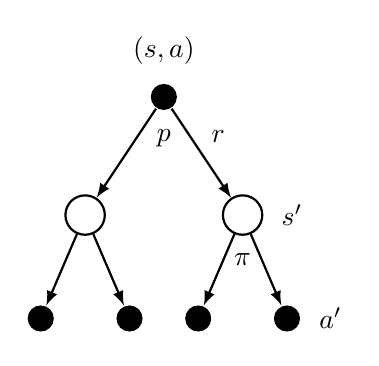
\begin{tikzpicture}[
>=latex, thick ,bend angle=8,auto,
state-node/.style = {circle,thick,draw=black,minimum size=5mm},
action-node/.style = {circle,fill=black, radius=2.5mm, minimum size=2.5mm}
]
   
\node [action-node] (root) at (0, 0) {};
\node [state-node] (l) at (-1, -1.5) {};
\node [state-node] (r) at (1, -1.5) {};
\node [action-node, below left=1cm and 0.25cm of l] (ll) {};
\node [action-node, below right=1cm and 0.25cm of l] (lr) {};
\node [action-node, below left=1cm and 0.25cm of r] (rl) {};
\node [action-node, below right=1cm and 0.25cm of r] (rr) {};

% labels
\node [above=1mm of root] {$(s, a)$};
\node [below=1mm of root] {$p$};
\node [right=1mm of r] {$s'$};
\node [below=1mm of r] {$\pi$};
\node [right=1mm of rr] {$a'$};

% arrows
\draw[->] (root) -- (l);
\draw[->] (root) -- node[midway]{$r$} (r);
\draw[->] (l) -- (ll);
\draw[->] (l) -- (lr);
\draw[->] (r) -- (rl);
\draw[->] (r) -- (rr);


\end{tikzpicture}
\caption{$q_\pi$ backup diagram}
\label{bellman_eq_action_val}
\end{figure}

\paragraph{\textit{Exercise 3.18} (p. 62)} The value of a state depends on the values of the actions possible in that state and on how likely each action is to be taken under the current policy. We can
think of this in terms of a small backup diagram rooted at the state and considering each
possible action:

\begin{figure}[h]
\centering
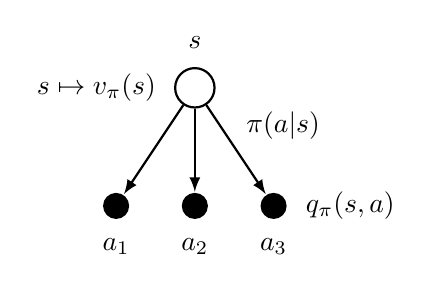
\begin{tikzpicture}[
>=latex, thick ,bend angle=8,auto,
state-node/.style = {circle,thick,draw=black,minimum size=5mm},
action-node/.style = {circle,fill=black, radius=2.5mm, minimum size=2.5mm}
]
   
\node [state-node] (root) at (0, 0) {};
\node [action-node] (l) at (-1, -1.5) {};
\node [action-node] (m) at (0, -1.5) {};
\node [action-node] (r) at (1, -1.5) {};


% labels
\node [above=1mm of root] {$s$};
\node [left=1mm of root] {$s \mapsto v_\pi(s)$};
\node [right=1mm of r] {$q_\pi(s, a)$};
\node [below=1mm of l] {$a_1$};
\node [below=1mm of m] {$a_2$};
\node [below=1mm of r] {$a_3$};


% arrows
\draw[->] (root) -- (l);
\draw[->] (root) -- (m);
\draw[->] (root) -- node[midway]{$\pi(a | s)$} (r);


\end{tikzpicture}
\caption{Small backup diagram showing $v_\pi$ in terms of $q_\pi$ and the policy $\pi$}
\label{relation_state_value_action_value}
\end{figure}


Give the equation corresponding to this intuition and diagram for the value at the root node, $v_\pi(s)$, in terms of the value at the expected leaf node, $q_\pi(s, a)$, given $S_t = s$. This equation should include an expectation conditioned on following the policy, $\pi$. Then give
a second equation in which the expected value is written out explicitly in terms of $\pi(a|s)$ such that no expected value notation appears in the equation.

\clearpage
\paragraph{\textit{Exercise 3.19} (p. 62)} The value of an action, $q_\pi(s, a)$, depends on the expected next reward and
the expected sum of the remaining rewards. Again we can think of this in terms of a
small backup diagram, this one rooted at an action (state-action pair) and branching to
the possible next states:

\begin{figure}[h]
\centering
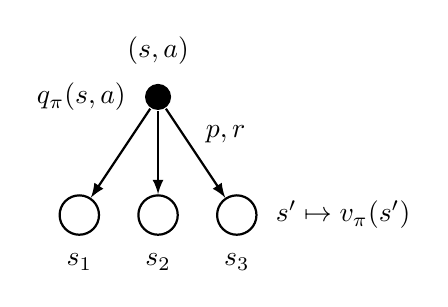
\begin{tikzpicture}[
>=latex, thick ,bend angle=8,auto,
state-node/.style = {circle,thick,draw=black,minimum size=5mm},
action-node/.style = {circle,fill=black, radius=2.5mm, minimum size=2.5mm}
]
   
\node [action-node] (root) at (0, 0) {};
\node [state-node] (l) at (-1, -1.5) {};
\node [state-node] (m) at (0, -1.5) {};
\node [state-node] (r) at (1, -1.5) {};

% labels
\node [above=1mm of root] {$(s, a)$};
\node [left=1mm of root] {$q_\pi(s, a)$};
\node [right=1mm of r] {$s' \mapsto v_\pi(s')$};
\node [below=1mm of l] {$s_1$};
\node [below=1mm of m] {$s_2$};
\node [below=1mm of r] {$s_3$};

% arrows
\draw[->] (root) -- (l);
\draw[->] (root) -- (m);
\draw[->] (root) -- node[midway]{$p, r$} (r);


\end{tikzpicture}
\caption{Small backup diagram showing $q_\pi$ in terms of $v_\pi$ and the dynamics function $p$}
\label{relation_action_value_state_value}
\end{figure}


Give the equation corresponding to this intuition and diagram for the action value, $q_\pi(s, a)$, in terms of the expected next reward, $R_{t+1}$, and the expected next state value, $v_\pi(St+1)$, given that $S_t=s$ and $A_t=a$. This equation should include an expectation but
\textit{not} one conditioned on following the policy.
Then give a second equation, writing out the expected value explicitly in terms of $p(s', r \lvert s, a)$ defined by ($3.2$), such that no expected value notation appears in the equation.

\paragraph{\textit{Exercise 3.20} (p. 66)} 
Draw or describe the optimal state-value function for the golf example.

\paragraph{\textit{Exercise 3.21} (p. 66)} 
Draw or describe the contours of the optimal action-value function for
putting, $q_*(s, \textrm{\textbf{putter}})$, for the golf example.

\paragraph{\textit{Exercise 3.22} (p. 66)} 

Consider the continuing MDP shown in Figure \ref{mdp_transition_graph}. The only decision to be made is that in the top state, where two actions are available, \textbf{left} and \textbf{right}. The numbers show the rewards that are received deterministically after each action. There are exactly two deterministic policies,
$\pi_\textrm{left}$ and $\pi_\textrm{right}$. What policy is optimal if $\gamma = 0$? If $\gamma = 0.9$?
If $\gamma = 0.5$?

\begin{figure}[h!]
\centering
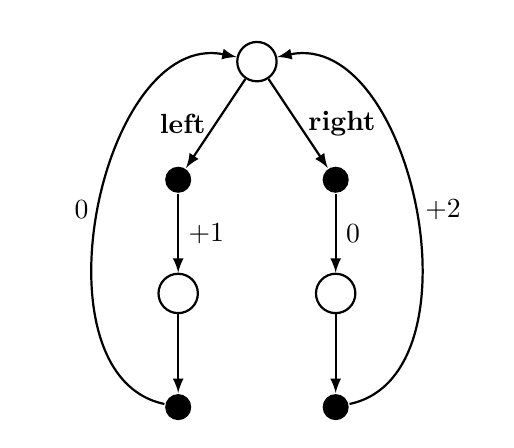
\begin{tikzpicture}[
>=latex, thick ,bend angle=90,
state-node/.style = {circle,thick,draw=black,minimum size=5mm},
action-node/.style = {circle,fill=black, radius=2.5mm, minimum size=2.5mm}
]
   
\node [state-node] (root) at (0, 0) {};
\node [action-node] (l) at (-1, -1.5) {};
\node [action-node] (r) at (1, -1.5) {};

\node [state-node, below=1cm of l] (lmstate) {};
\node [state-node, below=1cm of r] (rmstate) {};

\node [action-node, below=1cm of lmstate] (lm) {};
\node [action-node, below=1cm of rmstate] (rm) {};


% arrows
\draw[->] (root) -- node[midway, left]{\textbf{left}} (l);
\draw[->] (root) -- node[midway, right]{\textbf{right}} (r);
\draw[->] (l) -- node[midway, right]{$+1$} (lmstate);
\draw[->] (r) -- node[midway, right]{$0$} (rmstate);
\draw[->] (lmstate) -- node[midway, left]{} (lm);
\draw[->] (rmstate) -- node[midway, right]{} (rm);

\draw[->] (lm) edge [bend left] node[midway, left]{$0$} (root);
\draw[->] (rm) edge [bend right] node[midway, right]{$+2$} (root);


\end{tikzpicture}
\caption{MDP transition graph}
\label{mdp_transition_graph}
\end{figure}

\paragraph{\textit{Exercise 3.23} (p. 67)} Give the Bellman equation for $q_*$ for the recycling robot.

\paragraph{\textit{Exercise 3.24} (p. 67)} Figure $3.5$ (Gridworld) gives the optimal value of the best state of the gridworld as $24.4$, to one decimal place. Use your knowledge of the optimal policy and ($3.8$) to express this value symbolically, and then to compute it to three decimal places.

\clearpage
\paragraph{\textit{Exercise 3.25} (p. 67)} Give an equation for $v_*$ in terms of $q_*$.

\bigskip
From page $63$ of the book, "Intuitively, the Bellman optimality equation expresses the
fact that the value of a state under an optimal policy must equal the expected return for
the best action from that state"

\begin{equation}
v_*(s) = \sum_{a} \pi(a \lvert s) q_*(s, a) = \max_{a} q_*(s, a)
\end{equation}

where $a \in \mathcal{A}(s)$

\paragraph{\textit{Exercise 3.26} (p. 67)} Give an equation for $q_*$ in terms of $v_*$ and the four-argument $p$.

\bigskip
\begin{equation}
q_*(s, a) = \sum_{s', r} p(s', r \lvert s, a) \left[r + \gamma v_*(s')\right]
\end{equation}

\paragraph{\textit{Exercise 3.27} (p. 67)} Give an equation for $\pi_*$ in terms of $q_*$.

\bigskip

From page $68$ of the book, "Any policy that is greedy with respect to the optimal value functions must be an optimal
policy." and from page $65$, "With $q_*$ the agent does not
even have to do a one-step-ahead search: for any state $s$, it can simply find any action
that maximizes $q_*(s, a)$", translating it into a formula gives us one possible optimal value function:

\begin{equation}
\pi_*(a \lvert s) = \begin{cases} 1 & \textrm{if } a = \argmax\limits_{a'} q_*(s, a')\\ 0 & \textrm{else}\end{cases}
\end{equation}

if we suppose that the argmax gives one of the maximizing actions if many actions achieve the maximum.

\paragraph{\textit{Exercise 3.28} (p. 67)} Give an equation for $\pi_*$ in terms of $v_*$ and the four-argument $p$.

\bigskip
By using the previous exercise and Exercise $3.26$ where
\begin{equation}
q_*(s, a') = \sum_{s', r} p(s', r \lvert s, a') \left[r + \gamma v_*(s')\right]
\end{equation}

we get

\begin{equation}
\pi_*(a \lvert s) = \begin{cases} 1 & \textrm{if } a = \argmax\limits_{a'} \sum_{s', r} p(s', r \lvert s, a') \left[r + \gamma v_*(s')\right] \\ 0 & \textrm{else}\end{cases}
\end{equation}

\paragraph{\textit{Exercise 3.29} (p. 67)} Rewrite the four Bellman equations for the four value functions ($v_\pi$, $v_*$, $q_\pi$,
and $q_*$) in terms of the three argument function $p$ ($3.4$) and the two-argument function $r$
($3.5$).

\bigskip
Let's just first recall how to obtain the three argument function $p$ and the two-argument function $r$ from the $4$ argument function $p$ describing the MDP dynamics:

\begin{equation}
p(s' \lvert s, a) \doteq \sum_{r \in \mathcal{R}} p(s', r \lvert s, a)
\end{equation}

\begin{equation}
r(s, a) \doteq \mathbb{E}[R_{t+1} \lvert S_t = s, A_t= a] = \sum_{r \in \mathcal{R}} r \cdot p(r \lvert s, a) = \sum_{r \in \mathcal{R}} r \sum_{s' \in \mathcal{S}} p(s', r \lvert s, a)
\end{equation}

We can also recall the $4$ Bellman equations for the four value functions:
\begin{equation}
v_\pi(s) = \sum_{a} \pi(a \lvert s) \sum_{s', r} p(s', r \lvert s, a) \left[r + \gamma v_\pi(s')\right]
\end{equation}

\begin{equation}
v_*(s) = \max_{a} \sum_{s', r} p(s', r \lvert s, a) \left[r + \gamma v_*(s')\right]
\end{equation}

\begin{equation}
q_\pi(s, a) = \sum_{s', r} p(s', r \lvert s, a) \left[r + \gamma \sum_{a'} \pi(a' \lvert s') q_\pi(s', a')\right]
\end{equation}

\begin{equation}
q_*(s, a) = \sum_{s', r} p(s', r \lvert s, a) \left[r + \gamma \max_{a'} q_*(s', a')\right]
\end{equation}


where $a \in \mathcal{A}(s)$, $s'$ and $s \in \mathcal{S}$ and $r \in \mathcal{R}$. By replacing all the $4$ Bellman equations with ($3.4$) and ($3.5$) from the book:

\begin{equation}
v_\pi(s) = \sum_{a} \pi(a \lvert s) \left[ r(s, a) + \gamma \sum_{s'} p(s' \lvert s, a) v_\pi(s')\right]
\end{equation}

\begin{equation}
v_*(s) = \max_{a} \left\{ r(s, a) + \gamma \sum_{s'} p(s' \lvert s, a) v_*(s') \right\}
\end{equation}


\begin{equation}
q_\pi(s, a) = r(s, a) + \gamma \sum_{s'} p(s' \lvert s, a) \sum_{a'} \pi(a' \lvert s') q_\pi(s', a')
\end{equation}

\begin{equation}
q_*(s, a) = r(s, a) + \gamma \sum_{s'} p(s' \lvert s, a) \max_{a'} q_*(s', a')
\end{equation}

As remark, the Bellman equation with two-argument function $r$ and three-argument  function $p$ could be used directly to obtain the last equality for $v_*(\textrm{\textbf{h}})$ or the equation for $v_*(\textrm{\textbf{l}})$ in Example $3.9$ on the Bellman Optimality Equation for Recycling Robot (p. 65).

\paragraph{Proof of the formula used in the first equality of Example $3.9$ Bellman Optimality Equation for Recycling Robot (p. 65)}

We want to prove that 
\begin{equation}
v_*(s) = \max_{a} \sum_{s'} p(s' \lvert s, a) \left[r(s, a, s') + \gamma v_*(s')\right]
\end{equation}

Recall the definition of $r(s, a, s')$ that is the expected reward for state--action--next-state triples (($3.6$) in the book at page $49$)
\begin{equation}
\begin{split}
r(s, a, s') \doteq \mathbb{E}[R_{t+1} \lvert S_t = s, A_t = a, S_{t+1} = s'] &= \sum_{r \in \mathcal{R}} r \cdot p(r \lvert s, a, s')\\
&= \sum_{r \in \mathcal{R}} r \cdot \frac{p(s', r \lvert s, a)}{p(s' \lvert s, a)}
\end{split}
\end{equation}

And this gives us $\sum_{s'} p(s' \lvert s, a) \cdot r(s, a, s') = \sum_{s', r} r \cdot p(s', r \lvert s, a)$ and we substitute it in the Bellman equation for $v_*$.

\begin{equation}
\begin{split}
v_*(s) &= \max_{a} \sum_{s', r} p(s', r \lvert s, a) \left[r + \gamma v_*(s')\right]\\
&=\max_{a}\left\{\sum_{s'} p(s' \lvert s, a) \cdot r(s, a, s') + \gamma \sum_{s', r} p(s', r \lvert s, a) v_*(s')\right\}\\
&= \max_{a} \sum_{s'} p(s' \lvert s, a) \left[r(s, a, s') + \gamma v_*(s')\right]
\end{split}
\end{equation}

This proves the formula.

\end{document}